%\section{Theoritical expressive power of \EPMNModel{} and \LPMN{}}

\label{sec:equivalence}



In this section, we establish the relationship between different \EPModels{} and \LPModels{} models with respect to their theoretical expressive power. We consider single attribute (one user and one object attribute) and multi-attribute \EPModels{} and \LPModels{} models. A relationship among these models is  schematically presented in Figure \ref{fig:all-equivalence}. On the left and right side of the Y-axis, we present single attribute and multi-attribute  models respectively. On above and below the X-axis, we present enumerated and logical-formula policy models respectively. In all these models, we only consider set valued attributes. On the other hand, policy tuples are represented differently in \EPOneOneModels{} and \EPMNModel{} models. While the former uses atomic values (e.g. $(manager,TS)$),  the later uses set values (e.g. $(\{manager\}\,\{TS\})$) in a policy tuple.

We establish four different equivalences labeled number one to four in Figure \ref{fig:all-equivalence}. The first  equivalence  shows  that single and multi attribute \EPModels{} models are equivalent whereas the third equivalence shows similar result for  \LPModels{} models. The second equivalence shows that multi-attribute \EPModels{} models are as expressive as multi-attribute \LPModels{} models. The fourth equivalence shows similar result for single attribute. 



\textbf{Equivalence of single and multi attribute EAP models:}  We follow the foundation of  \cite{tripli}   to establish the equivalence of theoretical expressive power, referred to \TL{} equivalence for convenience. \TL{} requires us to define an access control model as an access control scheme of state transition system, present the mappings between the models in concern and show the mappings satisfy the requirements of state matching reduction. Additionally, we need to specify the access control queries that we need to preserve in the equivalence. 

%The mappings between \EPMNModel{} and \EPOneOneModels{} are presented in Table \ref{tab:mapping-epmn-ep11}.

% Representation of the model in TripLi schema and proof of state matching reduction are shown in the appendix. Note that, in the reductions, we do not consider state transitions for addition/deletion  of users, objects, authorization policies, and attribute-value assignments. We consider \clabac{} model presented in \cite{labac} as \EPOneOneModels{}.

We consider \clabac{} model presented in \cite{labac} as \EPOneOneModels{}. We present \EPOneOneModels{} in \TL{} as ($\myGamma{1,1}, \myQ{1,1}, \myvdash{1,1}, \myPSI{1,1}$) where a state,  $ \mygamma{}{1,1} \in \myGamma{1,1}$ is  specified as$(U, O, A, S, uLabel, oLabel,$ $ \sessionLabels{},  UL,$  $ OL, \Policy)$. The queries are specified as $\myQ{1,1}=\{ \myq{sao}{1,1} \equiv \isAuthorized(s, a, o)|$  $ a\in A, s \in S, o \in O \}$. The set of state transition rules $\myPSI{1,1}$ are $\{\createSession,$ $ \assignValues,$ $ \removeValues, \deleteSession\}$. Finally, the entailment function is defined as $\mygamma{}{1,1} \myvdash{1,1} \myq{sao}{1,1}$ iff $\isAuthorized(s,a,o)$ $=true$.

\EPMNModel{}  is defined as ($\myGamma{m,n}, \myQ{m,n}, \myvdash{m,n},\myPSI{m,n}$ ) where  a state $ \mygamma{}{m,n} \in \myGamma{m,n}$ is specified as  $(U, O, A, S, \uLabelP{1},..\uLabelP{m}, \oLabelP{1},..\oLabel{n},$ $ \sessionLabelsP{1},..\sessionLabelsP{m},  \UL{1},..\UL{m},$  $ \OL{1},..\OL{n}, \Policy)$. The queries  $\myQ{m,n}=\{ \myq{sao}{m,n} \equiv \isAuthorized$ $(s, a, o) \}$.  State transition rules are represented as $\myPSI{m,n} =  \{\createSession,$ $ \assignValues,$ $ \removeValues, \deleteSession\}$. Finally, $\mygamma{}{m,n} \myvdash{m,n} \myq{sao}{m,n}$ iff $\isAuthorized(s,a,o)$ $=true$.

%\vspace{-1em}
\newcommand{\denom}{\empty}
\newcommand{\suffix}{\empty}
\newcommand{\suffixTwo}{\empty}
\begin{table}
	\centering
	\caption{ Mapping from \EPMNModel{} to \EPOneOneModels{} and vice versa } %\vspace*{3pt}
	\label{tab:mapping-epmn-ep11}
	\begin{tabular}{|l|}						
		\hline					
			\multicolumn{1}{|c|}{\underline{\textit{I. \EPOneOneModels{}  components}}} \\
			-  $U_{\suffix}, O_{\suffix},  A_{\suffix}, S_{\suffix}, UL_{\suffix}$, $OL_{\suffix}$ (users, objects, actions, sessions, user and object attribute values) \\ 				  
			-  $\uLabel_{\suffix}: U_{\suffix} \to 2^{UL_{\suffix}}$, $\oLabel_{\suffix}: O_{\suffix} \to 2^{OL_{\suffix}}$; $\creator_{\suffix}: S_{\suffix} \to U_{\suffix}$; $\sessionLabels_{\suffix}: S_{\suffix} \to 2^{UL_{\suffix}}$ \\
			- $\Policy_{a_{1,1}} \subseteq {UL_{\suffix}} \times {OL_{\suffix}}$, policy for action $a \in A$ and $\Policy_{1,1} = \{Policy_{a_{1,1}}| a \in A\}$\\
		   
	 \multicolumn{1}{|c|}{\underline{\textit{II. From \EPMNModel{} to \EPOneOneModels{}}}}\\	
			- $U = U_\denom{}, O = O_\denom{}, A = A_\denom{}, S_{\suffixTwo{}} = S$ \\
			- $UL = 2^{\UL{1}} \times 2^{\UL{2}} \times ... \times 2^{\UL{m}}$; $OL = 2^{\OL{1}} \times 2^{\OL{2}} \times ... \times 2^{\OL{m}}$\\  
			- $\uLabel(u) = 2^{\uLabelP{1}(u)} \times 2^{\uLabelP{2}(u)} \times ... \times 2^{\uLabelP{m}(u)} $\\
			- $\oLabel(u) = 2^{\oLabelP{1}(o)} \times 2^{\oLabelP{2}(o)} \times ... \times 2^{\oLabelP{n}(o)} $ \\
		
			- $\creator_{\suffixTwo}(s) = \creator(s)$; $\sessionLabels_{\suffixTwo{}}(s) = 2^{\sessionLabelsP{1}(s)} \times 2^{\sessionLabelsP{2}(s)} \times ... \times 2^{\sessionLabelsP{m}(s)}$\\
			
			-  $\Policy_{a_{1,1}}= \{( (\ULS{1},  \ULS{2}, ..., \ULS{m}),  (\OLS{1}, \OLS{2}, ..., \OLS{n}))|$ \\ \hfill $(\exists (\ULS{1}, \ULS{2}, ...,\ULS{m},  \OLS{1}, \OLS{2}, ...,\OLS{n}) \in \Policy_a  )$ $[ \Policy_a \in \Policy_{m,n}]\}$ \\
			\multicolumn{1}{|c|}{\underline{\textit{III. From \EPOneOneModels{} to \EPMNModel{}}}}\\	
			
				- $U = U_\denom, O = O_\denom, A = A_\denom, S_{\suffixTwo} = S$ \\
				- $\UL{1} = UL$, $\UL{i} = \{\}$, for $2\le i \le m$; $\OL{1} = OL$, $\OL{i} = \{\}$, for $2\le i \le n$\\
				- $\uLabelP{1}(u) = \uLabelP{}(u)$, $\uLabelP{i}(u) = \{\}$, for $2 \le i  \le m $\\
				- $\oLabelP{1}(o) = \oLabelP{}(o)$, $\oLabelP{i}(o) = \{\}$, for $2 \le i  \le n $\\
				- $\creator(s) = \creator(s)$, for $s \in S$; $\sessionLabelsP{1}(s) = \sessionLabelsP{}(s)$, $\sessionLabelsP{i}(s) = \{\}$, for $2 \le i \le m$\\
				- $\Policy_a = \{( \{ul\}, \{\}, ...\{\}, \{ol\}, \{\}, ... \{\} ) | (ul,ol) \in \Policy_{a_{1,1}}[ \Policy_{a_{1,1}} \in \Policy_{1,1}]\}$\\
		 \hline	
	\end{tabular}	

	
\end{table}
%\vspace{-1em}
% 
 	\begin{figure} 
 		\centering
 		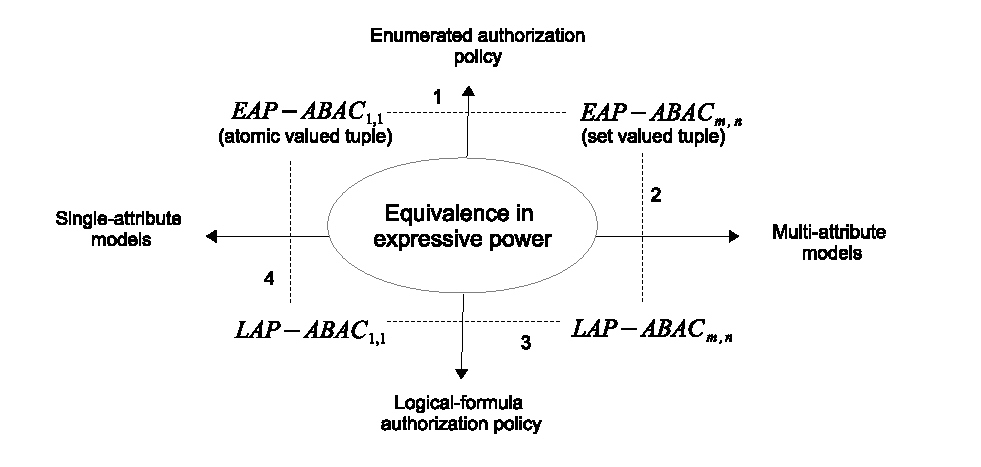
\includegraphics[width=.9\textwidth]{DBSEC16/all-equivalence}
 		\caption{Equilavence of enumerated and logical-formula auth. policy ABAC models}
 		\label{fig:all-equivalence}
 	\end{figure}
 




%While, the former uses $m$ user  and $n$ object attributes, the later uses only one user and one object attribute. Additionally, \EPOneOneModels{} uses atomic valued tuples and \EPMNModel{} uses set valued tuples.

%For each element in the result of the cartesian product, we define a value of the single user attribute. 

The mappings between \EPMNModel{} and \EPOneOneModels{} are presented in Table \ref{tab:mapping-epmn-ep11}. Segment I  presents the \EPOneOneModels{} model \cite{labac}. In  Segment II, we show the mapping from  \EPMNModel{} to \EPOneOneModels{}.  To combine $m$ user attributes of \EPMNModel{} into single attribute  of \EPOneOneModels{}, we take a cross product of the ranges of all $m$ attributes. To map set valued policy tuple into atomic valued policy tuple, we consider power set of the attribute values in computing the cross product.  We follow the similar process in computing single object attribute  and session-label values.  Finally, a tuple of \textit{m} user and \textit{n} object attribute values is converted to a 2-valued-tuple where the first value comes from $m$ user attributes and the second value comes from $n$ object attributes. The second mapping from \EPOneOneModels{} to \EPMNModel{}, given in Segment III, is straightforward where we use only one user and one object attribute out of $m$ and $n$ attributes. 



To show the mappings satisfy the requirements of state matching transition, let $\mygamma{0}{1,1}$ and $\mygamma{0}{m,n}$ be the start state of \EPOneOneModels{} and \EPMNModel{}  respectively. Let $\mygamma{0}{1,1} \myvdash{1,1} \myq{sao}{1,1}$. i.e. $ \isAuthorized(s,a,o) = true$ and thus, $(ul,ol) \in \Policy_a$, $ul \in uLabel(u)$ and  $ol \in oLabel(o)$ in $\mygamma{0}{1,1}$. According to Segment III of the mapping, it also happens that $(\{ul\},\{\}... \{ol\}.. \{\}) \in \Policy_a$, $ul \in uLabel(u)$ and  $ol \in oLabel(o)$ in $\mygamma{0}{m,n}$. Thus, $\mygamma{0}{m,n} \myvdash{m,n} \myq{0}{m,n}$. So, the initial states are equivalent. Now, for each state transition in $\myPSI{1,1}$ there also exists a similar transition in $\myPSI{m,n}$. For example, $\createSession$ exists in both $\myPSI{1,1}$ and $\myPSI{m,n}$. So, whenever, \EPOneOneModels{} reaches a new state using its state transition rules, so does \EPMNModel{}. So, there exists a one-to-one mapping between states of both models. We can use the same arguments as for initial states to show that corresponding states of the two models are equivalent. This proves the mapping from \EPOneOneModels{} to \EPMNModel{} is a state matching reduction. Similarly, we can show the same result holds for the other mapping. Thus, \EPOneOneModels{} and \EPMNModel{} are equivalent in expressive power.

%\vspace{-1em}
 
\begin{table}[t]
	\centering
	\caption{ Mapping from \EPMNModel{} to \LPMN{} and vice versa } %\vspace*{3pt}
	\label{tab:mapping-epmn-lpmn}
	\begin{tabular}{|l|}						
		\hline					
				   
			 \multicolumn{1}{|c|}{\underline{\textit{I. From \EPMNModel{} to \LPMN{}}}}\\	
				 - $\UAV{i} = \UL{i}$, for $ 1 \le i \le m$; $\OAV{i} = \OL{i}$, for $ 1 \le i \le n$\\
				 - $\ua{i}(u) = \uLabelP{i}(u)$; $\oa{i}(o) = \oLabelP{i}(o)$; $\sa{i}(s) = \sessionLabelsP{i}(s)$\\
				 - $\creator(s) = \creator(s)$;  $ f_a =$ \\
				  $\mathop{\bigvee}\limits_{ ( \ULS{1}, \ULS{2},..\ULS{m}, \OLS{1}, \OLS{2},..,\OLS{n}) \in \policy_a}  (\mathop{\wedge}\limits_{ 1 \le i \le m } \ULS{i} \subseteq \sa{i}(u) ) \wedge ( \mathop{\wedge}\limits_{ 1 \le i \le n } \OLS{i} \subseteq \oa{i}(u)$ \\

			\multicolumn{1}{|c|}{\underline{\textit{II. From \LPMN{} to \EPMNModel{}}}}\\	
			
				- $\UL{i} = \UAV{i}$, for $ 1 \le i \le m$ ; $\OL{i} = \OAV{i}$, for $ 1 \le i \le n$\\
				- $\uLabelP{i}(u) = \ua{i}(u)$, $\sessionLabelsP{i}(u) = \sa{i}(s)$ for $ 1 \le i \le m$; $\oLabelP{i}(o) = \oa{i}(o)$, for $ 1 \le i \le n$\\
			    -  $\creator(s) = \creator(s)$\\ 
			    - $\Policy_a = \{ ( \ULS{1}, \ULS{2}, ..., \ULS{m}, \OLS{1}, \OLS{2}, ..., \OLS{n}) |$ \\ \hfill $ f_a( \ULS{1}, \ULS{2}, ..., \ULS{m}, \OLS{1}, \OLS{2}, ..., \OLS{n}) = true \}$\\
			 
		 \hline	
	\end{tabular}	

	
\end{table}
%\vspace{-1em}
%\vspace{-1em}
\renewcommand{\suffix}{m,n}
\newcommand{\suffixT}{1,1}
\begin{table}
	\centering
	\caption{ Mappings } %\vspace*{3pt}
	\label{tab:lp11-to-lpmn}
	\begin{tabular}{|l|}						
		\hline					
%			\multicolumn{1}{|c|}{\underline{\textit{I. \LPOneOne{} components}}} \\
%				  - $U, O, A, S, UAV, OAV$  (users,  objects, actions, subjects, user and object attr. values.)\\
%				  - $ua,oa$ (attribute functions);  $ua:U\to 2^{UAV}$; $oa:O\to 2^{OAV}$ \\ 
%				  - $\subCreator: S \to U$ ; $sa:S\to 2^{UAV}$,    $sa(s) \subseteq ua(\subCreator(s))$\\
%				  - $f_a: (sa(u), oa(o)) \to \{true, false\}$  and $\isAuthorized(s,a,o) =(f_a(sa(u),oa(o))=true$) \\
				 
		   
		   \multicolumn{1}{|c|}{\underline{\textit{I. From \LPMN{} to \LPOneOne{}}}}\\	
			   - $U = U_{\suffix}; O = O_{\suffix}; A = A_{\suffix}; S = S_{\suffix};$$\textit{UAV} = \UAV{1} \times \UAV{2}\times ... \times \UAV{m}$\\
			   -  $\textit{OAV} = \OAV{1} \times \OAV{2}\times ... \times \OAV{m}$;$ua(u) = \ua{1}(u) \times \ua{2}(u) \times ... \times \ua{m}(u) $\\
			   -$oa(u) = \oa{1}(u) \times  ... \times \oa{m}(u) $$sa(u) = \sa{1}(u) \times ... \times \sa{m}(u) $; $\creator(s) = \creator_{\suffix}(s)$\\
			    - $ f_a =$ $\mathop{\bigvee}\limits_{ f_{a_{m,n}}( \ULS{1}, \ULS{2},...\ULS{m}, \OLS{1}, \OLS{2}, ...,\OLS{n})=true }  (\ULS{1}(u) \times ... \times \ULS{m}(u) \subseteq ua(u) )\land$ \\ \hfill  $(\OLS{1}(o) \times ... \times \OLS{n}(o) \subseteq oa(o))$, for $\ULS{i} \subseteq \UAV{i}$ and $\OLS{i} \subseteq \OAV{i}$ \\ 		
			   
 
	   \multicolumn{1}{|c|}{\underline{\textit{II. From \LPOneOne{} to \LPMN{}}}}\\	
			- $U = U_{\suffixT}; O = O_{\suffixT}; A = A_{\suffixT}; S = S_{\suffixT};$\\
			- $\UAV{1} = UAV; \UAV{2} = \{\}; ... \UAV{m} = \{\};$  $\OAV{1} = OAV; \OAV{2} = \{\}; ... \OAV{n} = \{\};$\\
			- $\ua{1}(u) = ua(u); \ua{2}(u) = \{\};...\ua{m}(u) = \{\}$; $\oa{1}(o) = oa(o); \oa{2}(o) = \{\};...\oa{m}(o) = \{\}$\\
		    - $\sa{1}(u) = sa(u); \sa{2}(u) = \{\};...\sa{m}(u) = \{\}$; $\creator_{\suffix}(s) = \creator(s)$ and $f_{a_{\suffix}} =$\\
		    $\mathop{\bigvee}\limits_{ f_{a}( \ULS{i},\OLS{i})=true }  (\ULS{i} \subseteq \ua{1}(u) \land$   $ \OLS{i}\subseteq oa(o))$  for $\ULS{i} \subseteq UAV$ and $\OLS{i} \subseteq OAV$ \\ 
		 %\hline	
		 	\multicolumn{1}{|c|}{\underline{\textit{III. From \EPOneOneModels{} to \LPOneOne{} }}}\\					
		 	- $U  = U ; O  = O ; A  = A $; $UAV	= UL; OAV = OL$;$ua(u) = uLabel(u)$; $oa(o)=oLabel(o) $\\
		 	-  $sa(s) = \sessionLabels(s) $ ;$f_a =$ $\mathop{\vee}\limits_{ (ul_i, ol_i) \in \policy_a} ( ul_i \in ua(u) \land ol_i \in oa(o))$. \\
		 	
		 	\multicolumn{1}{|c|}{\underline{\textit{IV. From \LPOneOne{} to \EPOneOneModels{}}}}\\	
		 	- $UL= 2^{ULV}; OL= 2^{OLV}; \uLabel(u) = 2^{ua(u)};\oLabel(o) = 2^{oa(o)}; \sessionLabels(s) = 2^{sa(s)}$ \\	  
		 	- $\Policy_a = \{  (\ulsubset, \olsubset) | (\exists \ulsubset \subseteq UL, \exists \olsubset \subseteq OL)[ f_a(\ulsubset, o\ulsubset) = true] \} $
		 	
		 	\\ \hline	
	\end{tabular}	

	
\end{table}
%\vspace{-1.5em}

\textbf{\textit{Equivalence of multi-attribute EAP and LAP models:}} Segment I and Segment II of Table \ref{tab:mapping-epmn-lpmn} show the required mapping from \EPMNModel{} to  \LPMN{} and  vice versa. In the mappings, both models have \textit{m} user and \textit{n} object attributes. Attributes values, and attribute value assignments and sessions  of one model are mapped to that of the other model. In Segment I, while generating a logical-formula policy from enumerated tuples, for each tuple we build an attribute value expression. Multiple tuples are matched with multiple expression connected by logical $\lor$ operators. In building an expression, for each set of values  in the tuple, we check if the values are activated in the session or contained by corresponding object attribute. On the other hand, in building tuples from a logical formula, for the sets of values of each attribute that evaluate the formula true, we create one tuple for  these values. For brevity, we do not show the \TL{} representation for this and later equivalences. Mappings for  the equivalences between \LPOneOne{} and \LPMN{} \& \LPOneOne{} and \EPOneOneModels{}  are given in Table \ref{tab:lp11-to-lpmn}.





